% Created by tikzDevice version 0.6.2-92-0ad2792 on 2013-03-04 16:59:26
% !TEX encoding = UTF-8 Unicode
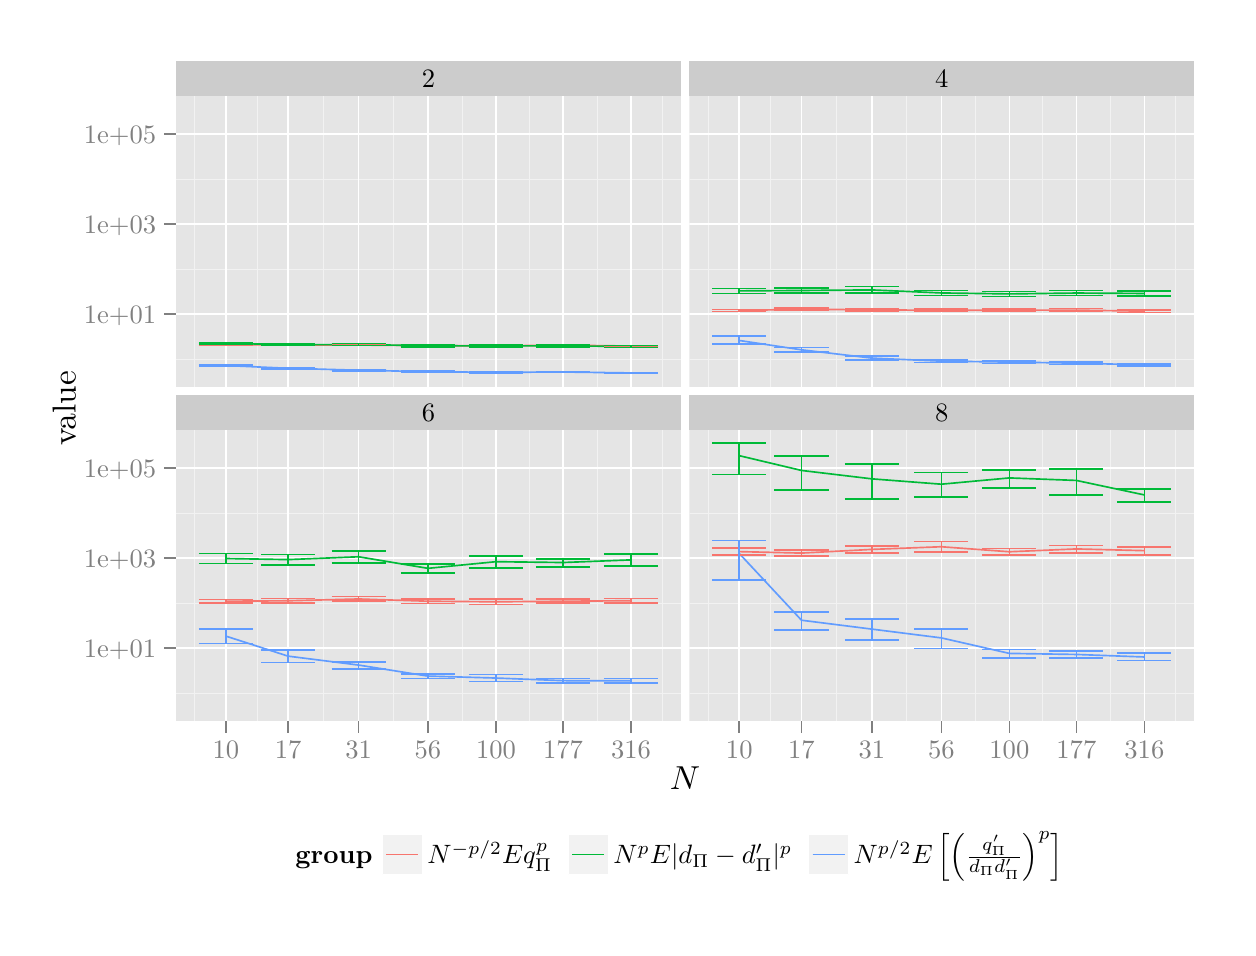
\begin{tikzpicture}[x=1pt,y=1pt]
\definecolor[named]{fillColor}{rgb}{1.00,1.00,1.00}
\path[use as bounding box,fill=fillColor,fill opacity=0.00] (0,0) rectangle (433.62,325.21);
\begin{scope}
\path[clip] (  0.00,  0.00) rectangle (433.62,325.21);
\definecolor[named]{drawColor}{rgb}{1.00,1.00,1.00}
\definecolor[named]{fillColor}{rgb}{1.00,1.00,1.00}

\path[draw=drawColor,line width= 0.6pt,line join=round,line cap=round,fill=fillColor] (  0.00,  0.00) rectangle (433.62,325.21);
\end{scope}
\begin{scope}
\path[clip] ( 53.55,195.47) rectangle (236.06,300.54);
\definecolor[named]{fillColor}{rgb}{0.90,0.90,0.90}

\path[fill=fillColor] ( 53.55,195.47) rectangle (236.06,300.54);
\definecolor[named]{drawColor}{rgb}{0.95,0.95,0.95}

\path[draw=drawColor,line width= 0.3pt,line join=round] ( 53.55,205.46) --
	(236.06,205.46);

\path[draw=drawColor,line width= 0.3pt,line join=round] ( 53.55,237.97) --
	(236.06,237.97);

\path[draw=drawColor,line width= 0.3pt,line join=round] ( 53.55,270.48) --
	(236.06,270.48);

\path[draw=drawColor,line width= 0.3pt,line join=round] ( 60.36,195.47) --
	( 60.36,300.54);

\path[draw=drawColor,line width= 0.3pt,line join=round] ( 82.85,195.47) --
	( 82.85,300.54);

\path[draw=drawColor,line width= 0.3pt,line join=round] (106.84,195.47) --
	(106.84,300.54);

\path[draw=drawColor,line width= 0.3pt,line join=round] (132.11,195.47) --
	(132.11,300.54);

\path[draw=drawColor,line width= 0.3pt,line join=round] (156.93,195.47) --
	(156.93,300.54);

\path[draw=drawColor,line width= 0.3pt,line join=round] (181.33,195.47) --
	(181.33,300.54);

\path[draw=drawColor,line width= 0.3pt,line join=round] (205.71,195.47) --
	(205.71,300.54);

\path[draw=drawColor,line width= 0.3pt,line join=round] (229.25,195.47) --
	(229.25,300.54);
\definecolor[named]{drawColor}{rgb}{1.00,1.00,1.00}

\path[draw=drawColor,line width= 0.6pt,line join=round] ( 53.55,221.71) --
	(236.06,221.71);

\path[draw=drawColor,line width= 0.6pt,line join=round] ( 53.55,254.22) --
	(236.06,254.22);

\path[draw=drawColor,line width= 0.6pt,line join=round] ( 53.55,286.73) --
	(236.06,286.73);

\path[draw=drawColor,line width= 0.6pt,line join=round] ( 71.61,195.47) --
	( 71.61,300.54);

\path[draw=drawColor,line width= 0.6pt,line join=round] ( 94.10,195.47) --
	( 94.10,300.54);

\path[draw=drawColor,line width= 0.6pt,line join=round] (119.57,195.47) --
	(119.57,300.54);

\path[draw=drawColor,line width= 0.6pt,line join=round] (144.64,195.47) --
	(144.64,300.54);

\path[draw=drawColor,line width= 0.6pt,line join=round] (169.22,195.47) --
	(169.22,300.54);

\path[draw=drawColor,line width= 0.6pt,line join=round] (193.43,195.47) --
	(193.43,300.54);

\path[draw=drawColor,line width= 0.6pt,line join=round] (218.00,195.47) --
	(218.00,300.54);
\definecolor[named]{drawColor}{rgb}{0.97,0.46,0.43}

\path[draw=drawColor,line width= 0.6pt,line join=round] ( 71.61,210.76) --
	( 94.10,210.52) --
	(119.57,210.52) --
	(144.64,210.30) --
	(169.22,210.22) --
	(193.43,210.48) --
	(218.00,210.17);
\definecolor[named]{drawColor}{rgb}{0.00,0.73,0.22}

\path[draw=drawColor,line width= 0.6pt,line join=round] ( 71.61,211.16) --
	( 94.10,210.65) --
	(119.57,210.71) --
	(144.64,210.28) --
	(169.22,210.19) --
	(193.43,210.25) --
	(218.00,209.99);
\definecolor[named]{drawColor}{rgb}{0.38,0.61,1.00}

\path[draw=drawColor,line width= 0.6pt,line join=round] ( 71.61,203.12) --
	( 94.10,202.13) --
	(119.57,201.43) --
	(144.64,200.89) --
	(169.22,200.66) --
	(193.43,200.78) --
	(218.00,200.45);
\definecolor[named]{drawColor}{rgb}{0.97,0.46,0.43}

\path[draw=drawColor,line width= 0.6pt,line join=round] ( 61.85,210.94) --
	( 81.37,210.94);

\path[draw=drawColor,line width= 0.6pt,line join=round] ( 71.61,210.94) --
	( 71.61,210.57);

\path[draw=drawColor,line width= 0.6pt,line join=round] ( 61.85,210.57) --
	( 81.37,210.57);

\path[draw=drawColor,line width= 0.6pt,line join=round] ( 84.34,210.70) --
	(103.86,210.70);

\path[draw=drawColor,line width= 0.6pt,line join=round] ( 94.10,210.70) --
	( 94.10,210.32);

\path[draw=drawColor,line width= 0.6pt,line join=round] ( 84.34,210.32) --
	(103.86,210.32);

\path[draw=drawColor,line width= 0.6pt,line join=round] (109.81,210.70) --
	(129.33,210.70);

\path[draw=drawColor,line width= 0.6pt,line join=round] (119.57,210.70) --
	(119.57,210.32);

\path[draw=drawColor,line width= 0.6pt,line join=round] (109.81,210.32) --
	(129.33,210.32);

\path[draw=drawColor,line width= 0.6pt,line join=round] (134.88,210.49) --
	(154.40,210.49);

\path[draw=drawColor,line width= 0.6pt,line join=round] (144.64,210.49) --
	(144.64,210.11);

\path[draw=drawColor,line width= 0.6pt,line join=round] (134.88,210.11) --
	(154.40,210.11);

\path[draw=drawColor,line width= 0.6pt,line join=round] (159.46,210.42) --
	(178.98,210.42);

\path[draw=drawColor,line width= 0.6pt,line join=round] (169.22,210.42) --
	(169.22,210.02);

\path[draw=drawColor,line width= 0.6pt,line join=round] (159.46,210.02) --
	(178.98,210.02);

\path[draw=drawColor,line width= 0.6pt,line join=round] (183.67,210.68) --
	(203.19,210.68);

\path[draw=drawColor,line width= 0.6pt,line join=round] (193.43,210.68) --
	(193.43,210.28);

\path[draw=drawColor,line width= 0.6pt,line join=round] (183.67,210.28) --
	(203.19,210.28);

\path[draw=drawColor,line width= 0.6pt,line join=round] (208.24,210.37) --
	(227.76,210.37);

\path[draw=drawColor,line width= 0.6pt,line join=round] (218.00,210.37) --
	(218.00,209.97);

\path[draw=drawColor,line width= 0.6pt,line join=round] (208.24,209.97) --
	(227.76,209.97);
\definecolor[named]{drawColor}{rgb}{0.00,0.73,0.22}

\path[draw=drawColor,line width= 0.6pt,line join=round] ( 61.85,211.50) --
	( 81.37,211.50);

\path[draw=drawColor,line width= 0.6pt,line join=round] ( 71.61,211.50) --
	( 71.61,210.83);

\path[draw=drawColor,line width= 0.6pt,line join=round] ( 61.85,210.83) --
	( 81.37,210.83);

\path[draw=drawColor,line width= 0.6pt,line join=round] ( 84.34,211.01) --
	(103.86,211.01);

\path[draw=drawColor,line width= 0.6pt,line join=round] ( 94.10,211.01) --
	( 94.10,210.32);

\path[draw=drawColor,line width= 0.6pt,line join=round] ( 84.34,210.32) --
	(103.86,210.32);

\path[draw=drawColor,line width= 0.6pt,line join=round] (109.81,211.09) --
	(129.33,211.09);

\path[draw=drawColor,line width= 0.6pt,line join=round] (119.57,211.09) --
	(119.57,210.33);

\path[draw=drawColor,line width= 0.6pt,line join=round] (109.81,210.33) --
	(129.33,210.33);

\path[draw=drawColor,line width= 0.6pt,line join=round] (134.88,210.61) --
	(154.40,210.61);

\path[draw=drawColor,line width= 0.6pt,line join=round] (144.64,210.61) --
	(144.64,209.93);

\path[draw=drawColor,line width= 0.6pt,line join=round] (134.88,209.93) --
	(154.40,209.93);

\path[draw=drawColor,line width= 0.6pt,line join=round] (159.46,210.53) --
	(178.98,210.53);

\path[draw=drawColor,line width= 0.6pt,line join=round] (169.22,210.53) --
	(169.22,209.85);

\path[draw=drawColor,line width= 0.6pt,line join=round] (159.46,209.85) --
	(178.98,209.85);

\path[draw=drawColor,line width= 0.6pt,line join=round] (183.67,210.60) --
	(203.19,210.60);

\path[draw=drawColor,line width= 0.6pt,line join=round] (193.43,210.60) --
	(193.43,209.92);

\path[draw=drawColor,line width= 0.6pt,line join=round] (183.67,209.92) --
	(203.19,209.92);

\path[draw=drawColor,line width= 0.6pt,line join=round] (208.24,210.30) --
	(227.76,210.30);

\path[draw=drawColor,line width= 0.6pt,line join=round] (218.00,210.30) --
	(218.00,209.65);

\path[draw=drawColor,line width= 0.6pt,line join=round] (208.24,209.65) --
	(227.76,209.65);
\definecolor[named]{drawColor}{rgb}{0.38,0.61,1.00}

\path[draw=drawColor,line width= 0.6pt,line join=round] ( 61.85,203.39) --
	( 81.37,203.39);

\path[draw=drawColor,line width= 0.6pt,line join=round] ( 71.61,203.39) --
	( 71.61,202.84);

\path[draw=drawColor,line width= 0.6pt,line join=round] ( 61.85,202.84) --
	( 81.37,202.84);

\path[draw=drawColor,line width= 0.6pt,line join=round] ( 84.34,202.37) --
	(103.86,202.37);

\path[draw=drawColor,line width= 0.6pt,line join=round] ( 94.10,202.37) --
	( 94.10,201.89);

\path[draw=drawColor,line width= 0.6pt,line join=round] ( 84.34,201.89) --
	(103.86,201.89);

\path[draw=drawColor,line width= 0.6pt,line join=round] (109.81,201.64) --
	(129.33,201.64);

\path[draw=drawColor,line width= 0.6pt,line join=round] (119.57,201.64) --
	(119.57,201.20);

\path[draw=drawColor,line width= 0.6pt,line join=round] (109.81,201.20) --
	(129.33,201.20);

\path[draw=drawColor,line width= 0.6pt,line join=round] (134.88,201.10) --
	(154.40,201.10);

\path[draw=drawColor,line width= 0.6pt,line join=round] (144.64,201.10) --
	(144.64,200.70);

\path[draw=drawColor,line width= 0.6pt,line join=round] (134.88,200.70) --
	(154.40,200.70);

\path[draw=drawColor,line width= 0.6pt,line join=round] (159.46,200.88) --
	(178.98,200.88);

\path[draw=drawColor,line width= 0.6pt,line join=round] (169.22,200.88) --
	(169.22,200.47);

\path[draw=drawColor,line width= 0.6pt,line join=round] (159.46,200.47) --
	(178.98,200.47);

\path[draw=drawColor,line width= 0.6pt,line join=round] (183.67,200.99) --
	(203.19,200.99);

\path[draw=drawColor,line width= 0.6pt,line join=round] (193.43,200.99) --
	(193.43,200.58);

\path[draw=drawColor,line width= 0.6pt,line join=round] (183.67,200.58) --
	(203.19,200.58);

\path[draw=drawColor,line width= 0.6pt,line join=round] (208.24,200.64) --
	(227.76,200.64);

\path[draw=drawColor,line width= 0.6pt,line join=round] (218.00,200.64) --
	(218.00,200.25);

\path[draw=drawColor,line width= 0.6pt,line join=round] (208.24,200.25) --
	(227.76,200.25);
\end{scope}
\begin{scope}
\path[clip] (239.07,195.47) rectangle (421.58,300.54);
\definecolor[named]{fillColor}{rgb}{0.90,0.90,0.90}

\path[fill=fillColor] (239.07,195.47) rectangle (421.57,300.54);
\definecolor[named]{drawColor}{rgb}{0.95,0.95,0.95}

\path[draw=drawColor,line width= 0.3pt,line join=round] (239.07,205.46) --
	(421.58,205.46);

\path[draw=drawColor,line width= 0.3pt,line join=round] (239.07,237.97) --
	(421.58,237.97);

\path[draw=drawColor,line width= 0.3pt,line join=round] (239.07,270.48) --
	(421.58,270.48);

\path[draw=drawColor,line width= 0.3pt,line join=round] (245.88,195.47) --
	(245.88,300.54);

\path[draw=drawColor,line width= 0.3pt,line join=round] (268.37,195.47) --
	(268.37,300.54);

\path[draw=drawColor,line width= 0.3pt,line join=round] (292.36,195.47) --
	(292.36,300.54);

\path[draw=drawColor,line width= 0.3pt,line join=round] (317.62,195.47) --
	(317.62,300.54);

\path[draw=drawColor,line width= 0.3pt,line join=round] (342.45,195.47) --
	(342.45,300.54);

\path[draw=drawColor,line width= 0.3pt,line join=round] (366.84,195.47) --
	(366.84,300.54);

\path[draw=drawColor,line width= 0.3pt,line join=round] (391.23,195.47) --
	(391.23,300.54);

\path[draw=drawColor,line width= 0.3pt,line join=round] (414.77,195.47) --
	(414.77,300.54);
\definecolor[named]{drawColor}{rgb}{1.00,1.00,1.00}

\path[draw=drawColor,line width= 0.6pt,line join=round] (239.07,221.71) --
	(421.58,221.71);

\path[draw=drawColor,line width= 0.6pt,line join=round] (239.07,254.22) --
	(421.58,254.22);

\path[draw=drawColor,line width= 0.6pt,line join=round] (239.07,286.73) --
	(421.58,286.73);

\path[draw=drawColor,line width= 0.6pt,line join=round] (257.13,195.47) --
	(257.13,300.54);

\path[draw=drawColor,line width= 0.6pt,line join=round] (279.62,195.47) --
	(279.62,300.54);

\path[draw=drawColor,line width= 0.6pt,line join=round] (305.09,195.47) --
	(305.09,300.54);

\path[draw=drawColor,line width= 0.6pt,line join=round] (330.16,195.47) --
	(330.16,300.54);

\path[draw=drawColor,line width= 0.6pt,line join=round] (354.74,195.47) --
	(354.74,300.54);

\path[draw=drawColor,line width= 0.6pt,line join=round] (378.95,195.47) --
	(378.95,300.54);

\path[draw=drawColor,line width= 0.6pt,line join=round] (403.52,195.47) --
	(403.52,300.54);
\definecolor[named]{drawColor}{rgb}{0.97,0.46,0.43}

\path[draw=drawColor,line width= 0.6pt,line join=round] (257.13,223.04) --
	(279.62,223.43) --
	(305.09,223.28) --
	(330.16,223.04) --
	(354.74,223.14) --
	(378.95,223.14) --
	(403.52,222.77);
\definecolor[named]{drawColor}{rgb}{0.00,0.73,0.22}

\path[draw=drawColor,line width= 0.6pt,line join=round] (257.13,230.10) --
	(279.62,230.24) --
	(305.09,230.44) --
	(330.16,229.35) --
	(354.74,229.00) --
	(378.95,229.32) --
	(403.52,229.16);
\definecolor[named]{drawColor}{rgb}{0.38,0.61,1.00}

\path[draw=drawColor,line width= 0.6pt,line join=round] (257.13,212.17) --
	(279.62,208.80) --
	(305.09,205.80) --
	(330.16,204.70) --
	(354.74,204.37) --
	(378.95,203.98) --
	(403.52,203.36);
\definecolor[named]{drawColor}{rgb}{0.97,0.46,0.43}

\path[draw=drawColor,line width= 0.6pt,line join=round] (247.36,223.40) --
	(266.89,223.40);

\path[draw=drawColor,line width= 0.6pt,line join=round] (257.13,223.40) --
	(257.13,222.64);

\path[draw=drawColor,line width= 0.6pt,line join=round] (247.36,222.64) --
	(266.89,222.64);

\path[draw=drawColor,line width= 0.6pt,line join=round] (269.86,223.86) --
	(289.38,223.86);

\path[draw=drawColor,line width= 0.6pt,line join=round] (279.62,223.86) --
	(279.62,222.99);

\path[draw=drawColor,line width= 0.6pt,line join=round] (269.86,222.99) --
	(289.38,222.99);

\path[draw=drawColor,line width= 0.6pt,line join=round] (295.33,223.73) --
	(314.85,223.73);

\path[draw=drawColor,line width= 0.6pt,line join=round] (305.09,223.73) --
	(305.09,222.84);

\path[draw=drawColor,line width= 0.6pt,line join=round] (295.33,222.84) --
	(314.85,222.84);

\path[draw=drawColor,line width= 0.6pt,line join=round] (320.40,223.48) --
	(339.92,223.48);

\path[draw=drawColor,line width= 0.6pt,line join=round] (330.16,223.48) --
	(330.16,222.60);

\path[draw=drawColor,line width= 0.6pt,line join=round] (320.40,222.60) --
	(339.92,222.60);

\path[draw=drawColor,line width= 0.6pt,line join=round] (344.98,223.56) --
	(364.50,223.56);

\path[draw=drawColor,line width= 0.6pt,line join=round] (354.74,223.56) --
	(354.74,222.68);

\path[draw=drawColor,line width= 0.6pt,line join=round] (344.98,222.68) --
	(364.50,222.68);

\path[draw=drawColor,line width= 0.6pt,line join=round] (369.19,223.67) --
	(388.71,223.67);

\path[draw=drawColor,line width= 0.6pt,line join=round] (378.95,223.67) --
	(378.95,222.63);

\path[draw=drawColor,line width= 0.6pt,line join=round] (369.19,222.63) --
	(388.71,222.63);

\path[draw=drawColor,line width= 0.6pt,line join=round] (393.76,223.21) --
	(413.28,223.21);

\path[draw=drawColor,line width= 0.6pt,line join=round] (403.52,223.21) --
	(403.52,222.31);

\path[draw=drawColor,line width= 0.6pt,line join=round] (393.76,222.31) --
	(413.28,222.31);
\definecolor[named]{drawColor}{rgb}{0.00,0.73,0.22}

\path[draw=drawColor,line width= 0.6pt,line join=round] (247.36,230.99) --
	(266.89,230.99);

\path[draw=drawColor,line width= 0.6pt,line join=round] (257.13,230.99) --
	(257.13,229.17);

\path[draw=drawColor,line width= 0.6pt,line join=round] (247.36,229.17) --
	(266.89,229.17);

\path[draw=drawColor,line width= 0.6pt,line join=round] (269.86,231.19) --
	(289.38,231.19);

\path[draw=drawColor,line width= 0.6pt,line join=round] (279.62,231.19) --
	(279.62,229.24);

\path[draw=drawColor,line width= 0.6pt,line join=round] (269.86,229.24) --
	(289.38,229.24);

\path[draw=drawColor,line width= 0.6pt,line join=round] (295.33,231.62) --
	(314.85,231.62);

\path[draw=drawColor,line width= 0.6pt,line join=round] (305.09,231.62) --
	(305.09,229.36);

\path[draw=drawColor,line width= 0.6pt,line join=round] (295.33,229.36) --
	(314.85,229.36);

\path[draw=drawColor,line width= 0.6pt,line join=round] (320.40,230.24) --
	(339.92,230.24);

\path[draw=drawColor,line width= 0.6pt,line join=round] (330.16,230.24) --
	(330.16,228.42);

\path[draw=drawColor,line width= 0.6pt,line join=round] (320.40,228.42) --
	(339.92,228.42);

\path[draw=drawColor,line width= 0.6pt,line join=round] (344.98,229.87) --
	(364.50,229.87);

\path[draw=drawColor,line width= 0.6pt,line join=round] (354.74,229.87) --
	(354.74,228.04);

\path[draw=drawColor,line width= 0.6pt,line join=round] (344.98,228.04) --
	(364.50,228.04);

\path[draw=drawColor,line width= 0.6pt,line join=round] (369.19,230.19) --
	(388.71,230.19);

\path[draw=drawColor,line width= 0.6pt,line join=round] (378.95,230.19) --
	(378.95,228.42);

\path[draw=drawColor,line width= 0.6pt,line join=round] (369.19,228.42) --
	(388.71,228.42);

\path[draw=drawColor,line width= 0.6pt,line join=round] (393.76,230.16) --
	(413.28,230.16);

\path[draw=drawColor,line width= 0.6pt,line join=round] (403.52,230.16) --
	(403.52,228.15);

\path[draw=drawColor,line width= 0.6pt,line join=round] (393.76,228.15) --
	(413.28,228.15);
\definecolor[named]{drawColor}{rgb}{0.38,0.61,1.00}

\path[draw=drawColor,line width= 0.6pt,line join=round] (247.36,213.71) --
	(266.89,213.71);

\path[draw=drawColor,line width= 0.6pt,line join=round] (257.13,213.71) --
	(257.13,210.81);

\path[draw=drawColor,line width= 0.6pt,line join=round] (247.36,210.81) --
	(266.89,210.81);

\path[draw=drawColor,line width= 0.6pt,line join=round] (269.86,209.64) --
	(289.38,209.64);

\path[draw=drawColor,line width= 0.6pt,line join=round] (279.62,209.64) --
	(279.62,207.91);

\path[draw=drawColor,line width= 0.6pt,line join=round] (269.86,207.91) --
	(289.38,207.91);

\path[draw=drawColor,line width= 0.6pt,line join=round] (295.33,206.45) --
	(314.85,206.45);

\path[draw=drawColor,line width= 0.6pt,line join=round] (305.09,206.45) --
	(305.09,205.14);

\path[draw=drawColor,line width= 0.6pt,line join=round] (295.33,205.14) --
	(314.85,205.14);

\path[draw=drawColor,line width= 0.6pt,line join=round] (320.40,205.18) --
	(339.92,205.18);

\path[draw=drawColor,line width= 0.6pt,line join=round] (330.16,205.18) --
	(330.16,204.24);

\path[draw=drawColor,line width= 0.6pt,line join=round] (320.40,204.24) --
	(339.92,204.24);

\path[draw=drawColor,line width= 0.6pt,line join=round] (344.98,204.87) --
	(364.50,204.87);

\path[draw=drawColor,line width= 0.6pt,line join=round] (354.74,204.87) --
	(354.74,203.84);

\path[draw=drawColor,line width= 0.6pt,line join=round] (344.98,203.84) --
	(364.50,203.84);

\path[draw=drawColor,line width= 0.6pt,line join=round] (369.19,204.46) --
	(388.71,204.46);

\path[draw=drawColor,line width= 0.6pt,line join=round] (378.95,204.46) --
	(378.95,203.44);

\path[draw=drawColor,line width= 0.6pt,line join=round] (369.19,203.44) --
	(388.71,203.44);

\path[draw=drawColor,line width= 0.6pt,line join=round] (393.76,203.79) --
	(413.28,203.79);

\path[draw=drawColor,line width= 0.6pt,line join=round] (403.52,203.79) --
	(403.52,202.91);

\path[draw=drawColor,line width= 0.6pt,line join=round] (393.76,202.91) --
	(413.28,202.91);
\end{scope}
\begin{scope}
\path[clip] ( 53.55, 74.76) rectangle (236.06,179.83);
\definecolor[named]{fillColor}{rgb}{0.90,0.90,0.90}

\path[fill=fillColor] ( 53.55, 74.76) rectangle (236.06,179.83);
\definecolor[named]{drawColor}{rgb}{0.95,0.95,0.95}

\path[draw=drawColor,line width= 0.3pt,line join=round] ( 53.55, 84.75) --
	(236.06, 84.75);

\path[draw=drawColor,line width= 0.3pt,line join=round] ( 53.55,117.26) --
	(236.06,117.26);

\path[draw=drawColor,line width= 0.3pt,line join=round] ( 53.55,149.77) --
	(236.06,149.77);

\path[draw=drawColor,line width= 0.3pt,line join=round] ( 60.36, 74.76) --
	( 60.36,179.83);

\path[draw=drawColor,line width= 0.3pt,line join=round] ( 82.85, 74.76) --
	( 82.85,179.83);

\path[draw=drawColor,line width= 0.3pt,line join=round] (106.84, 74.76) --
	(106.84,179.83);

\path[draw=drawColor,line width= 0.3pt,line join=round] (132.11, 74.76) --
	(132.11,179.83);

\path[draw=drawColor,line width= 0.3pt,line join=round] (156.93, 74.76) --
	(156.93,179.83);

\path[draw=drawColor,line width= 0.3pt,line join=round] (181.33, 74.76) --
	(181.33,179.83);

\path[draw=drawColor,line width= 0.3pt,line join=round] (205.71, 74.76) --
	(205.71,179.83);

\path[draw=drawColor,line width= 0.3pt,line join=round] (229.25, 74.76) --
	(229.25,179.83);
\definecolor[named]{drawColor}{rgb}{1.00,1.00,1.00}

\path[draw=drawColor,line width= 0.6pt,line join=round] ( 53.55,101.00) --
	(236.06,101.00);

\path[draw=drawColor,line width= 0.6pt,line join=round] ( 53.55,133.51) --
	(236.06,133.51);

\path[draw=drawColor,line width= 0.6pt,line join=round] ( 53.55,166.02) --
	(236.06,166.02);

\path[draw=drawColor,line width= 0.6pt,line join=round] ( 71.61, 74.76) --
	( 71.61,179.83);

\path[draw=drawColor,line width= 0.6pt,line join=round] ( 94.10, 74.76) --
	( 94.10,179.83);

\path[draw=drawColor,line width= 0.6pt,line join=round] (119.57, 74.76) --
	(119.57,179.83);

\path[draw=drawColor,line width= 0.6pt,line join=round] (144.64, 74.76) --
	(144.64,179.83);

\path[draw=drawColor,line width= 0.6pt,line join=round] (169.22, 74.76) --
	(169.22,179.83);

\path[draw=drawColor,line width= 0.6pt,line join=round] (193.43, 74.76) --
	(193.43,179.83);

\path[draw=drawColor,line width= 0.6pt,line join=round] (218.00, 74.76) --
	(218.00,179.83);
\definecolor[named]{drawColor}{rgb}{0.97,0.46,0.43}

\path[draw=drawColor,line width= 0.6pt,line join=round] ( 71.61,117.97) --
	( 94.10,118.11) --
	(119.57,118.77) --
	(144.64,117.96) --
	(169.22,117.74) --
	(193.43,117.96) --
	(218.00,118.14);
\definecolor[named]{drawColor}{rgb}{0.00,0.73,0.22}

\path[draw=drawColor,line width= 0.6pt,line join=round] ( 71.61,133.39) --
	( 94.10,133.00) --
	(119.57,134.02) --
	(144.64,129.84) --
	(169.22,132.24) --
	(193.43,131.94) --
	(218.00,132.89);
\definecolor[named]{drawColor}{rgb}{0.38,0.61,1.00}

\path[draw=drawColor,line width= 0.6pt,line join=round] ( 71.61,105.35) --
	( 94.10, 98.11) --
	(119.57, 94.89) --
	(144.64, 90.90) --
	(169.22, 90.20) --
	(193.43, 89.25) --
	(218.00, 89.21);
\definecolor[named]{drawColor}{rgb}{0.97,0.46,0.43}

\path[draw=drawColor,line width= 0.6pt,line join=round] ( 61.85,118.58) --
	( 81.37,118.58);

\path[draw=drawColor,line width= 0.6pt,line join=round] ( 71.61,118.58) --
	( 71.61,117.31);

\path[draw=drawColor,line width= 0.6pt,line join=round] ( 61.85,117.31) --
	( 81.37,117.31);

\path[draw=drawColor,line width= 0.6pt,line join=round] ( 84.34,118.95) --
	(103.86,118.95);

\path[draw=drawColor,line width= 0.6pt,line join=round] ( 94.10,118.95) --
	( 94.10,117.32);

\path[draw=drawColor,line width= 0.6pt,line join=round] ( 84.34,117.32) --
	(103.86,117.32);

\path[draw=drawColor,line width= 0.6pt,line join=round] (109.81,119.62) --
	(129.33,119.62);

\path[draw=drawColor,line width= 0.6pt,line join=round] (119.57,119.62) --
	(119.57,117.97);

\path[draw=drawColor,line width= 0.6pt,line join=round] (109.81,117.97) --
	(129.33,117.97);

\path[draw=drawColor,line width= 0.6pt,line join=round] (134.88,118.68) --
	(154.40,118.68);

\path[draw=drawColor,line width= 0.6pt,line join=round] (144.64,118.68) --
	(144.64,117.18);

\path[draw=drawColor,line width= 0.6pt,line join=round] (134.88,117.18) --
	(154.40,117.18);

\path[draw=drawColor,line width= 0.6pt,line join=round] (159.46,118.71) --
	(178.98,118.71);

\path[draw=drawColor,line width= 0.6pt,line join=round] (169.22,118.71) --
	(169.22,116.74);

\path[draw=drawColor,line width= 0.6pt,line join=round] (159.46,116.74) --
	(178.98,116.74);

\path[draw=drawColor,line width= 0.6pt,line join=round] (183.67,118.69) --
	(203.19,118.69);

\path[draw=drawColor,line width= 0.6pt,line join=round] (193.43,118.69) --
	(193.43,117.27);

\path[draw=drawColor,line width= 0.6pt,line join=round] (183.67,117.27) --
	(203.19,117.27);

\path[draw=drawColor,line width= 0.6pt,line join=round] (208.24,118.96) --
	(227.76,118.96);

\path[draw=drawColor,line width= 0.6pt,line join=round] (218.00,118.96) --
	(218.00,117.28);

\path[draw=drawColor,line width= 0.6pt,line join=round] (208.24,117.28) --
	(227.76,117.28);
\definecolor[named]{drawColor}{rgb}{0.00,0.73,0.22}

\path[draw=drawColor,line width= 0.6pt,line join=round] ( 61.85,135.16) --
	( 81.37,135.16);

\path[draw=drawColor,line width= 0.6pt,line join=round] ( 71.61,135.16) --
	( 71.61,131.61);

\path[draw=drawColor,line width= 0.6pt,line join=round] ( 61.85,131.61) --
	( 81.37,131.61);

\path[draw=drawColor,line width= 0.6pt,line join=round] ( 84.34,134.82) --
	(103.86,134.82);

\path[draw=drawColor,line width= 0.6pt,line join=round] ( 94.10,134.82) --
	( 94.10,131.02);

\path[draw=drawColor,line width= 0.6pt,line join=round] ( 84.34,131.02) --
	(103.86,131.02);

\path[draw=drawColor,line width= 0.6pt,line join=round] (109.81,136.21) --
	(129.33,136.21);

\path[draw=drawColor,line width= 0.6pt,line join=round] (119.57,136.21) --
	(119.57,131.81);

\path[draw=drawColor,line width= 0.6pt,line join=round] (109.81,131.81) --
	(129.33,131.81);

\path[draw=drawColor,line width= 0.6pt,line join=round] (134.88,131.35) --
	(154.40,131.35);

\path[draw=drawColor,line width= 0.6pt,line join=round] (144.64,131.35) --
	(144.64,128.04);

\path[draw=drawColor,line width= 0.6pt,line join=round] (134.88,128.04) --
	(154.40,128.04);

\path[draw=drawColor,line width= 0.6pt,line join=round] (159.46,134.30) --
	(178.98,134.30);

\path[draw=drawColor,line width= 0.6pt,line join=round] (169.22,134.30) --
	(169.22,129.92);

\path[draw=drawColor,line width= 0.6pt,line join=round] (159.46,129.92) --
	(178.98,129.92);

\path[draw=drawColor,line width= 0.6pt,line join=round] (183.67,133.31) --
	(203.19,133.31);

\path[draw=drawColor,line width= 0.6pt,line join=round] (193.43,133.31) --
	(193.43,130.33);

\path[draw=drawColor,line width= 0.6pt,line join=round] (183.67,130.33) --
	(203.19,130.33);

\path[draw=drawColor,line width= 0.6pt,line join=round] (208.24,134.93) --
	(227.76,134.93);

\path[draw=drawColor,line width= 0.6pt,line join=round] (218.00,134.93) --
	(218.00,130.63);

\path[draw=drawColor,line width= 0.6pt,line join=round] (208.24,130.63) --
	(227.76,130.63);
\definecolor[named]{drawColor}{rgb}{0.38,0.61,1.00}

\path[draw=drawColor,line width= 0.6pt,line join=round] ( 61.85,107.87) --
	( 81.37,107.87);

\path[draw=drawColor,line width= 0.6pt,line join=round] ( 71.61,107.87) --
	( 71.61,102.66);

\path[draw=drawColor,line width= 0.6pt,line join=round] ( 61.85,102.66) --
	( 81.37,102.66);

\path[draw=drawColor,line width= 0.6pt,line join=round] ( 84.34,100.29) --
	(103.86,100.29);

\path[draw=drawColor,line width= 0.6pt,line join=round] ( 94.10,100.29) --
	( 94.10, 95.86);

\path[draw=drawColor,line width= 0.6pt,line join=round] ( 84.34, 95.86) --
	(103.86, 95.86);

\path[draw=drawColor,line width= 0.6pt,line join=round] (109.81, 96.11) --
	(129.33, 96.11);

\path[draw=drawColor,line width= 0.6pt,line join=round] (119.57, 96.11) --
	(119.57, 93.56);

\path[draw=drawColor,line width= 0.6pt,line join=round] (109.81, 93.56) --
	(129.33, 93.56);

\path[draw=drawColor,line width= 0.6pt,line join=round] (134.88, 91.72) --
	(154.40, 91.72);

\path[draw=drawColor,line width= 0.6pt,line join=round] (144.64, 91.72) --
	(144.64, 90.03);

\path[draw=drawColor,line width= 0.6pt,line join=round] (134.88, 90.03) --
	(154.40, 90.03);

\path[draw=drawColor,line width= 0.6pt,line join=round] (159.46, 91.53) --
	(178.98, 91.53);

\path[draw=drawColor,line width= 0.6pt,line join=round] (169.22, 91.53) --
	(169.22, 88.97);

\path[draw=drawColor,line width= 0.6pt,line join=round] (159.46, 88.97) --
	(178.98, 88.97);

\path[draw=drawColor,line width= 0.6pt,line join=round] (183.67, 90.02) --
	(203.19, 90.02);

\path[draw=drawColor,line width= 0.6pt,line join=round] (193.43, 90.02) --
	(193.43, 88.46);

\path[draw=drawColor,line width= 0.6pt,line join=round] (183.67, 88.46) --
	(203.19, 88.46);

\path[draw=drawColor,line width= 0.6pt,line join=round] (208.24, 89.99) --
	(227.76, 89.99);

\path[draw=drawColor,line width= 0.6pt,line join=round] (218.00, 89.99) --
	(218.00, 88.37);

\path[draw=drawColor,line width= 0.6pt,line join=round] (208.24, 88.37) --
	(227.76, 88.37);
\end{scope}
\begin{scope}
\path[clip] (239.07, 74.76) rectangle (421.58,179.83);
\definecolor[named]{fillColor}{rgb}{0.90,0.90,0.90}

\path[fill=fillColor] (239.07, 74.76) rectangle (421.57,179.83);
\definecolor[named]{drawColor}{rgb}{0.95,0.95,0.95}

\path[draw=drawColor,line width= 0.3pt,line join=round] (239.07, 84.75) --
	(421.58, 84.75);

\path[draw=drawColor,line width= 0.3pt,line join=round] (239.07,117.26) --
	(421.58,117.26);

\path[draw=drawColor,line width= 0.3pt,line join=round] (239.07,149.77) --
	(421.58,149.77);

\path[draw=drawColor,line width= 0.3pt,line join=round] (245.88, 74.76) --
	(245.88,179.83);

\path[draw=drawColor,line width= 0.3pt,line join=round] (268.37, 74.76) --
	(268.37,179.83);

\path[draw=drawColor,line width= 0.3pt,line join=round] (292.36, 74.76) --
	(292.36,179.83);

\path[draw=drawColor,line width= 0.3pt,line join=round] (317.62, 74.76) --
	(317.62,179.83);

\path[draw=drawColor,line width= 0.3pt,line join=round] (342.45, 74.76) --
	(342.45,179.83);

\path[draw=drawColor,line width= 0.3pt,line join=round] (366.84, 74.76) --
	(366.84,179.83);

\path[draw=drawColor,line width= 0.3pt,line join=round] (391.23, 74.76) --
	(391.23,179.83);

\path[draw=drawColor,line width= 0.3pt,line join=round] (414.77, 74.76) --
	(414.77,179.83);
\definecolor[named]{drawColor}{rgb}{1.00,1.00,1.00}

\path[draw=drawColor,line width= 0.6pt,line join=round] (239.07,101.00) --
	(421.58,101.00);

\path[draw=drawColor,line width= 0.6pt,line join=round] (239.07,133.51) --
	(421.58,133.51);

\path[draw=drawColor,line width= 0.6pt,line join=round] (239.07,166.02) --
	(421.58,166.02);

\path[draw=drawColor,line width= 0.6pt,line join=round] (257.13, 74.76) --
	(257.13,179.83);

\path[draw=drawColor,line width= 0.6pt,line join=round] (279.62, 74.76) --
	(279.62,179.83);

\path[draw=drawColor,line width= 0.6pt,line join=round] (305.09, 74.76) --
	(305.09,179.83);

\path[draw=drawColor,line width= 0.6pt,line join=round] (330.16, 74.76) --
	(330.16,179.83);

\path[draw=drawColor,line width= 0.6pt,line join=round] (354.74, 74.76) --
	(354.74,179.83);

\path[draw=drawColor,line width= 0.6pt,line join=round] (378.95, 74.76) --
	(378.95,179.83);

\path[draw=drawColor,line width= 0.6pt,line join=round] (403.52, 74.76) --
	(403.52,179.83);
\definecolor[named]{drawColor}{rgb}{0.97,0.46,0.43}

\path[draw=drawColor,line width= 0.6pt,line join=round] (257.13,135.88) --
	(279.62,135.35) --
	(305.09,136.68) --
	(330.16,137.64) --
	(354.74,135.83) --
	(378.95,136.85) --
	(403.52,136.23);
\definecolor[named]{drawColor}{rgb}{0.00,0.73,0.22}

\path[draw=drawColor,line width= 0.6pt,line join=round] (257.13,170.55) --
	(279.62,165.21) --
	(305.09,162.17) --
	(330.16,160.24) --
	(354.74,162.51) --
	(378.95,161.60) --
	(403.52,156.36);
\definecolor[named]{drawColor}{rgb}{0.38,0.61,1.00}

\path[draw=drawColor,line width= 0.6pt,line join=round] (257.13,135.21) --
	(279.62,111.09) --
	(305.09,107.87) --
	(330.16,104.70) --
	(354.74, 99.10) --
	(378.95, 98.72) --
	(403.52, 97.81);
\definecolor[named]{drawColor}{rgb}{0.97,0.46,0.43}

\path[draw=drawColor,line width= 0.6pt,line join=round] (247.36,137.19) --
	(266.89,137.19);

\path[draw=drawColor,line width= 0.6pt,line join=round] (257.13,137.19) --
	(257.13,134.63);

\path[draw=drawColor,line width= 0.6pt,line join=round] (247.36,134.63) --
	(266.89,134.63);

\path[draw=drawColor,line width= 0.6pt,line join=round] (269.86,136.42) --
	(289.38,136.42);

\path[draw=drawColor,line width= 0.6pt,line join=round] (279.62,136.42) --
	(279.62,134.27);

\path[draw=drawColor,line width= 0.6pt,line join=round] (269.86,134.27) --
	(289.38,134.27);

\path[draw=drawColor,line width= 0.6pt,line join=round] (295.33,137.96) --
	(314.85,137.96);

\path[draw=drawColor,line width= 0.6pt,line join=round] (305.09,137.96) --
	(305.09,135.37);

\path[draw=drawColor,line width= 0.6pt,line join=round] (295.33,135.37) --
	(314.85,135.37);

\path[draw=drawColor,line width= 0.6pt,line join=round] (320.40,139.50) --
	(339.92,139.50);

\path[draw=drawColor,line width= 0.6pt,line join=round] (330.16,139.50) --
	(330.16,135.66);

\path[draw=drawColor,line width= 0.6pt,line join=round] (320.40,135.66) --
	(339.92,135.66);

\path[draw=drawColor,line width= 0.6pt,line join=round] (344.98,137.04) --
	(364.50,137.04);

\path[draw=drawColor,line width= 0.6pt,line join=round] (354.74,137.04) --
	(354.74,134.64);

\path[draw=drawColor,line width= 0.6pt,line join=round] (344.98,134.64) --
	(364.50,134.64);

\path[draw=drawColor,line width= 0.6pt,line join=round] (369.19,138.08) --
	(388.71,138.08);

\path[draw=drawColor,line width= 0.6pt,line join=round] (378.95,138.08) --
	(378.95,135.43);

\path[draw=drawColor,line width= 0.6pt,line join=round] (369.19,135.43) --
	(388.71,135.43);

\path[draw=drawColor,line width= 0.6pt,line join=round] (393.76,137.58) --
	(413.28,137.58);

\path[draw=drawColor,line width= 0.6pt,line join=round] (403.52,137.58) --
	(403.52,134.71);

\path[draw=drawColor,line width= 0.6pt,line join=round] (393.76,134.71) --
	(413.28,134.71);
\definecolor[named]{drawColor}{rgb}{0.00,0.73,0.22}

\path[draw=drawColor,line width= 0.6pt,line join=round] (247.36,175.05) --
	(266.89,175.05);

\path[draw=drawColor,line width= 0.6pt,line join=round] (257.13,175.05) --
	(257.13,163.72);

\path[draw=drawColor,line width= 0.6pt,line join=round] (247.36,163.72) --
	(266.89,163.72);

\path[draw=drawColor,line width= 0.6pt,line join=round] (269.86,170.55) --
	(289.38,170.55);

\path[draw=drawColor,line width= 0.6pt,line join=round] (279.62,170.55) --
	(279.62,158.24);

\path[draw=drawColor,line width= 0.6pt,line join=round] (269.86,158.24) --
	(289.38,158.24);

\path[draw=drawColor,line width= 0.6pt,line join=round] (295.33,167.49) --
	(314.85,167.49);

\path[draw=drawColor,line width= 0.6pt,line join=round] (305.09,167.49) --
	(305.09,154.91);

\path[draw=drawColor,line width= 0.6pt,line join=round] (295.33,154.91) --
	(314.85,154.91);

\path[draw=drawColor,line width= 0.6pt,line join=round] (320.40,164.53) --
	(339.92,164.53);

\path[draw=drawColor,line width= 0.6pt,line join=round] (330.16,164.53) --
	(330.16,155.59);

\path[draw=drawColor,line width= 0.6pt,line join=round] (320.40,155.59) --
	(339.92,155.59);

\path[draw=drawColor,line width= 0.6pt,line join=round] (344.98,165.44) --
	(364.50,165.44);

\path[draw=drawColor,line width= 0.6pt,line join=round] (354.74,165.44) --
	(354.74,158.84);

\path[draw=drawColor,line width= 0.6pt,line join=round] (344.98,158.84) --
	(364.50,158.84);

\path[draw=drawColor,line width= 0.6pt,line join=round] (369.19,165.78) --
	(388.71,165.78);

\path[draw=drawColor,line width= 0.6pt,line join=round] (378.95,165.78) --
	(378.95,156.30);

\path[draw=drawColor,line width= 0.6pt,line join=round] (369.19,156.30) --
	(388.71,156.30);

\path[draw=drawColor,line width= 0.6pt,line join=round] (393.76,158.60) --
	(413.28,158.60);

\path[draw=drawColor,line width= 0.6pt,line join=round] (403.52,158.60) --
	(403.52,153.74);

\path[draw=drawColor,line width= 0.6pt,line join=round] (393.76,153.74) --
	(413.28,153.74);
\definecolor[named]{drawColor}{rgb}{0.38,0.61,1.00}

\path[draw=drawColor,line width= 0.6pt,line join=round] (247.36,139.92) --
	(266.89,139.92);

\path[draw=drawColor,line width= 0.6pt,line join=round] (257.13,139.92) --
	(257.13,125.72);

\path[draw=drawColor,line width= 0.6pt,line join=round] (247.36,125.72) --
	(266.89,125.72);

\path[draw=drawColor,line width= 0.6pt,line join=round] (269.86,114.04) --
	(289.38,114.04);

\path[draw=drawColor,line width= 0.6pt,line join=round] (279.62,114.04) --
	(279.62,107.64);

\path[draw=drawColor,line width= 0.6pt,line join=round] (269.86,107.64) --
	(289.38,107.64);

\path[draw=drawColor,line width= 0.6pt,line join=round] (295.33,111.49) --
	(314.85,111.49);

\path[draw=drawColor,line width= 0.6pt,line join=round] (305.09,111.49) --
	(305.09,103.83);

\path[draw=drawColor,line width= 0.6pt,line join=round] (295.33,103.83) --
	(314.85,103.83);

\path[draw=drawColor,line width= 0.6pt,line join=round] (320.40,108.00) --
	(339.92,108.00);

\path[draw=drawColor,line width= 0.6pt,line join=round] (330.16,108.00) --
	(330.16,100.88);

\path[draw=drawColor,line width= 0.6pt,line join=round] (320.40,100.88) --
	(339.92,100.88);

\path[draw=drawColor,line width= 0.6pt,line join=round] (344.98,100.47) --
	(364.50,100.47);

\path[draw=drawColor,line width= 0.6pt,line join=round] (354.74,100.47) --
	(354.74, 97.49);

\path[draw=drawColor,line width= 0.6pt,line join=round] (344.98, 97.49) --
	(364.50, 97.49);

\path[draw=drawColor,line width= 0.6pt,line join=round] (369.19, 99.99) --
	(388.71, 99.99);

\path[draw=drawColor,line width= 0.6pt,line join=round] (378.95, 99.99) --
	(378.95, 97.41);

\path[draw=drawColor,line width= 0.6pt,line join=round] (369.19, 97.41) --
	(388.71, 97.41);

\path[draw=drawColor,line width= 0.6pt,line join=round] (393.76, 99.20) --
	(413.28, 99.20);

\path[draw=drawColor,line width= 0.6pt,line join=round] (403.52, 99.20) --
	(403.52, 96.49);

\path[draw=drawColor,line width= 0.6pt,line join=round] (393.76, 96.49) --
	(413.28, 96.49);
\end{scope}
\begin{scope}
\path[clip] (  0.00,  0.00) rectangle (433.62,325.21);
\definecolor[named]{fillColor}{rgb}{0.80,0.80,0.80}

\path[fill=fillColor] ( 53.55,300.54) rectangle (236.06,313.17);
\definecolor[named]{drawColor}{rgb}{0.00,0.00,0.00}

\node[text=drawColor,anchor=base,inner sep=0pt, outer sep=0pt, scale=  0.96] at (144.80,303.55) {2};
\end{scope}
\begin{scope}
\path[clip] (  0.00,  0.00) rectangle (433.62,325.21);
\definecolor[named]{fillColor}{rgb}{0.80,0.80,0.80}

\path[fill=fillColor] (239.07,300.54) rectangle (421.57,313.17);
\definecolor[named]{drawColor}{rgb}{0.00,0.00,0.00}

\node[text=drawColor,anchor=base,inner sep=0pt, outer sep=0pt, scale=  0.96] at (330.32,303.55) {4};
\end{scope}
\begin{scope}
\path[clip] (  0.00,  0.00) rectangle (433.62,325.21);
\definecolor[named]{fillColor}{rgb}{0.80,0.80,0.80}

\path[fill=fillColor] ( 53.55,179.83) rectangle (236.06,192.46);
\definecolor[named]{drawColor}{rgb}{0.00,0.00,0.00}

\node[text=drawColor,anchor=base,inner sep=0pt, outer sep=0pt, scale=  0.96] at (144.80,182.84) {6};
\end{scope}
\begin{scope}
\path[clip] (  0.00,  0.00) rectangle (433.62,325.21);
\definecolor[named]{fillColor}{rgb}{0.80,0.80,0.80}

\path[fill=fillColor] (239.07,179.83) rectangle (421.57,192.46);
\definecolor[named]{drawColor}{rgb}{0.00,0.00,0.00}

\node[text=drawColor,anchor=base,inner sep=0pt, outer sep=0pt, scale=  0.96] at (330.32,182.84) {8};
\end{scope}
\begin{scope}
\path[clip] (  0.00,  0.00) rectangle (433.62,325.21);
\definecolor[named]{drawColor}{rgb}{0.50,0.50,0.50}

\node[text=drawColor,anchor=base east,inner sep=0pt, outer sep=0pt, scale=  0.96] at ( 46.44,218.41) {1e+01};

\node[text=drawColor,anchor=base east,inner sep=0pt, outer sep=0pt, scale=  0.96] at ( 46.44,250.92) {1e+03};

\node[text=drawColor,anchor=base east,inner sep=0pt, outer sep=0pt, scale=  0.96] at ( 46.44,283.42) {1e+05};
\end{scope}
\begin{scope}
\path[clip] (  0.00,  0.00) rectangle (433.62,325.21);
\definecolor[named]{drawColor}{rgb}{0.50,0.50,0.50}

\path[draw=drawColor,line width= 0.6pt,line join=round] ( 49.28,221.71) --
	( 53.55,221.71);

\path[draw=drawColor,line width= 0.6pt,line join=round] ( 49.28,254.22) --
	( 53.55,254.22);

\path[draw=drawColor,line width= 0.6pt,line join=round] ( 49.28,286.73) --
	( 53.55,286.73);
\end{scope}
\begin{scope}
\path[clip] (  0.00,  0.00) rectangle (433.62,325.21);
\definecolor[named]{drawColor}{rgb}{0.50,0.50,0.50}

\node[text=drawColor,anchor=base east,inner sep=0pt, outer sep=0pt, scale=  0.96] at ( 46.44, 97.70) {1e+01};

\node[text=drawColor,anchor=base east,inner sep=0pt, outer sep=0pt, scale=  0.96] at ( 46.44,130.21) {1e+03};

\node[text=drawColor,anchor=base east,inner sep=0pt, outer sep=0pt, scale=  0.96] at ( 46.44,162.71) {1e+05};
\end{scope}
\begin{scope}
\path[clip] (  0.00,  0.00) rectangle (433.62,325.21);
\definecolor[named]{drawColor}{rgb}{0.50,0.50,0.50}

\path[draw=drawColor,line width= 0.6pt,line join=round] ( 49.28,101.00) --
	( 53.55,101.00);

\path[draw=drawColor,line width= 0.6pt,line join=round] ( 49.28,133.51) --
	( 53.55,133.51);

\path[draw=drawColor,line width= 0.6pt,line join=round] ( 49.28,166.02) --
	( 53.55,166.02);
\end{scope}
\begin{scope}
\path[clip] (  0.00,  0.00) rectangle (433.62,325.21);
\definecolor[named]{drawColor}{rgb}{0.50,0.50,0.50}

\path[draw=drawColor,line width= 0.6pt,line join=round] ( 71.61, 70.49) --
	( 71.61, 74.76);

\path[draw=drawColor,line width= 0.6pt,line join=round] ( 94.10, 70.49) --
	( 94.10, 74.76);

\path[draw=drawColor,line width= 0.6pt,line join=round] (119.57, 70.49) --
	(119.57, 74.76);

\path[draw=drawColor,line width= 0.6pt,line join=round] (144.64, 70.49) --
	(144.64, 74.76);

\path[draw=drawColor,line width= 0.6pt,line join=round] (169.22, 70.49) --
	(169.22, 74.76);

\path[draw=drawColor,line width= 0.6pt,line join=round] (193.43, 70.49) --
	(193.43, 74.76);

\path[draw=drawColor,line width= 0.6pt,line join=round] (218.00, 70.49) --
	(218.00, 74.76);
\end{scope}
\begin{scope}
\path[clip] (  0.00,  0.00) rectangle (433.62,325.21);
\definecolor[named]{drawColor}{rgb}{0.50,0.50,0.50}

\node[text=drawColor,anchor=base,inner sep=0pt, outer sep=0pt, scale=  0.96] at ( 71.61, 61.03) {10};

\node[text=drawColor,anchor=base,inner sep=0pt, outer sep=0pt, scale=  0.96] at ( 94.10, 61.03) {17};

\node[text=drawColor,anchor=base,inner sep=0pt, outer sep=0pt, scale=  0.96] at (119.57, 61.03) {31};

\node[text=drawColor,anchor=base,inner sep=0pt, outer sep=0pt, scale=  0.96] at (144.64, 61.03) {56};

\node[text=drawColor,anchor=base,inner sep=0pt, outer sep=0pt, scale=  0.96] at (169.22, 61.03) {100};

\node[text=drawColor,anchor=base,inner sep=0pt, outer sep=0pt, scale=  0.96] at (193.43, 61.03) {177};

\node[text=drawColor,anchor=base,inner sep=0pt, outer sep=0pt, scale=  0.96] at (218.00, 61.03) {316};
\end{scope}
\begin{scope}
\path[clip] (  0.00,  0.00) rectangle (433.62,325.21);
\definecolor[named]{drawColor}{rgb}{0.50,0.50,0.50}

\path[draw=drawColor,line width= 0.6pt,line join=round] (257.13, 70.49) --
	(257.13, 74.76);

\path[draw=drawColor,line width= 0.6pt,line join=round] (279.62, 70.49) --
	(279.62, 74.76);

\path[draw=drawColor,line width= 0.6pt,line join=round] (305.09, 70.49) --
	(305.09, 74.76);

\path[draw=drawColor,line width= 0.6pt,line join=round] (330.16, 70.49) --
	(330.16, 74.76);

\path[draw=drawColor,line width= 0.6pt,line join=round] (354.74, 70.49) --
	(354.74, 74.76);

\path[draw=drawColor,line width= 0.6pt,line join=round] (378.95, 70.49) --
	(378.95, 74.76);

\path[draw=drawColor,line width= 0.6pt,line join=round] (403.52, 70.49) --
	(403.52, 74.76);
\end{scope}
\begin{scope}
\path[clip] (  0.00,  0.00) rectangle (433.62,325.21);
\definecolor[named]{drawColor}{rgb}{0.50,0.50,0.50}

\node[text=drawColor,anchor=base,inner sep=0pt, outer sep=0pt, scale=  0.96] at (257.13, 61.03) {10};

\node[text=drawColor,anchor=base,inner sep=0pt, outer sep=0pt, scale=  0.96] at (279.62, 61.03) {17};

\node[text=drawColor,anchor=base,inner sep=0pt, outer sep=0pt, scale=  0.96] at (305.09, 61.03) {31};

\node[text=drawColor,anchor=base,inner sep=0pt, outer sep=0pt, scale=  0.96] at (330.16, 61.03) {56};

\node[text=drawColor,anchor=base,inner sep=0pt, outer sep=0pt, scale=  0.96] at (354.74, 61.03) {100};

\node[text=drawColor,anchor=base,inner sep=0pt, outer sep=0pt, scale=  0.96] at (378.95, 61.03) {177};

\node[text=drawColor,anchor=base,inner sep=0pt, outer sep=0pt, scale=  0.96] at (403.52, 61.03) {316};
\end{scope}
\begin{scope}
\path[clip] (  0.00,  0.00) rectangle (433.62,325.21);
\definecolor[named]{drawColor}{rgb}{0.00,0.00,0.00}

\node[text=drawColor,anchor=base,inner sep=0pt, outer sep=0pt, scale=  1.20] at (237.56, 49.76) {$N$};
\end{scope}
\begin{scope}
\path[clip] (  0.00,  0.00) rectangle (433.62,325.21);
\definecolor[named]{drawColor}{rgb}{0.00,0.00,0.00}

\node[text=drawColor,rotate= 90.00,anchor=base,inner sep=0pt, outer sep=0pt, scale=  1.20] at ( 17.30,187.65) {value};
\end{scope}
\begin{scope}
\path[clip] (  0.00,  0.00) rectangle (433.62,325.21);
\definecolor[named]{fillColor}{rgb}{1.00,1.00,1.00}

\path[fill=fillColor] ( 92.48, 14.89) rectangle (382.65, 37.88);
\end{scope}
\begin{scope}
\path[clip] (  0.00,  0.00) rectangle (433.62,325.21);
\definecolor[named]{drawColor}{rgb}{0.00,0.00,0.00}

\node[text=drawColor,anchor=base west,inner sep=0pt, outer sep=0pt, scale=  0.96] at ( 96.75, 23.07) {\bfseries group};
\end{scope}
\begin{scope}
\path[clip] (  0.00,  0.00) rectangle (433.62,325.21);
\definecolor[named]{drawColor}{rgb}{1.00,1.00,1.00}
\definecolor[named]{fillColor}{rgb}{0.95,0.95,0.95}

\path[draw=drawColor,line width= 0.6pt,line join=round,line cap=round,fill=fillColor] (128.21, 19.16) rectangle (142.66, 33.61);
\end{scope}
\begin{scope}
\path[clip] (  0.00,  0.00) rectangle (433.62,325.21);
\definecolor[named]{drawColor}{rgb}{0.97,0.46,0.43}

\path[draw=drawColor,line width= 0.6pt,line join=round] (129.65, 26.39) -- (141.21, 26.39);
\end{scope}
\begin{scope}
\path[clip] (  0.00,  0.00) rectangle (433.62,325.21);
\definecolor[named]{drawColor}{rgb}{0.97,0.46,0.43}

\path[draw=drawColor,line width= 0.6pt,line join=round] (129.65, 26.39) -- (141.21, 26.39);
\end{scope}
\begin{scope}
\path[clip] (  0.00,  0.00) rectangle (433.62,325.21);
\definecolor[named]{drawColor}{rgb}{1.00,1.00,1.00}
\definecolor[named]{fillColor}{rgb}{0.95,0.95,0.95}

\path[draw=drawColor,line width= 0.6pt,line join=round,line cap=round,fill=fillColor] (195.40, 19.16) rectangle (209.85, 33.61);
\end{scope}
\begin{scope}
\path[clip] (  0.00,  0.00) rectangle (433.62,325.21);
\definecolor[named]{drawColor}{rgb}{0.00,0.73,0.22}

\path[draw=drawColor,line width= 0.6pt,line join=round] (196.84, 26.39) -- (208.41, 26.39);
\end{scope}
\begin{scope}
\path[clip] (  0.00,  0.00) rectangle (433.62,325.21);
\definecolor[named]{drawColor}{rgb}{0.00,0.73,0.22}

\path[draw=drawColor,line width= 0.6pt,line join=round] (196.84, 26.39) -- (208.41, 26.39);
\end{scope}
\begin{scope}
\path[clip] (  0.00,  0.00) rectangle (433.62,325.21);
\definecolor[named]{drawColor}{rgb}{1.00,1.00,1.00}
\definecolor[named]{fillColor}{rgb}{0.95,0.95,0.95}

\path[draw=drawColor,line width= 0.6pt,line join=round,line cap=round,fill=fillColor] (282.19, 19.16) rectangle (296.64, 33.61);
\end{scope}
\begin{scope}
\path[clip] (  0.00,  0.00) rectangle (433.62,325.21);
\definecolor[named]{drawColor}{rgb}{0.38,0.61,1.00}

\path[draw=drawColor,line width= 0.6pt,line join=round] (283.63, 26.39) -- (295.19, 26.39);
\end{scope}
\begin{scope}
\path[clip] (  0.00,  0.00) rectangle (433.62,325.21);
\definecolor[named]{drawColor}{rgb}{0.38,0.61,1.00}

\path[draw=drawColor,line width= 0.6pt,line join=round] (283.63, 26.39) -- (295.19, 26.39);
\end{scope}
\begin{scope}
\path[clip] (  0.00,  0.00) rectangle (433.62,325.21);
\definecolor[named]{drawColor}{rgb}{0.00,0.00,0.00}

\node[text=drawColor,anchor=base west,inner sep=0pt, outer sep=0pt, scale=  0.96] at (144.47, 23.08) {$N^{-p/2}\mathbb{E} q_{\Pi}^p \;\;$};
\end{scope}
\begin{scope}
\path[clip] (  0.00,  0.00) rectangle (433.62,325.21);
\definecolor[named]{drawColor}{rgb}{0.00,0.00,0.00}

\node[text=drawColor,anchor=base west,inner sep=0pt, outer sep=0pt, scale=  0.96] at (211.66, 23.08) {$N^{p}\mathbb{E}|d_{\Pi}-d'_{\Pi}|^p\;\;$};
\end{scope}
\begin{scope}
\path[clip] (  0.00,  0.00) rectangle (433.62,325.21);
\definecolor[named]{drawColor}{rgb}{0.00,0.00,0.00}

\node[text=drawColor,anchor=base west,inner sep=0pt, outer sep=0pt, scale=  0.96] at (298.45, 23.08) {$N^{p/2}\mathbb{E}\left [ \left ( \frac{q'_{\Pi}}{d_{\Pi}d'_{\Pi}} \right ) ^p \right ]\;\;$};
\end{scope}
\end{tikzpicture}
